\chapter{Background} \label{ch:background}

\section{Submodularity} \label{sect:bg_submod}

Modeling notions such as coverage, representativeness, or diversity is an important challenge in many machine learning problems.
These notions are well captured by submodular set functions.
Analogously, supermodular functions capture notions of smoothness, regularity, or cooperation. 
As a result, submodularity and supermodularity have found numerous applications in machine learning problems of discrete nature, akin to concavity and convexity for continuous optimization.

\subsection{Basics}
We consider set functions $F : 2^V \to \mathbb{R}$, where $V$ is a finite ground set of size $|V| = n$.
Without loss of generality, if not otherwise stated, we will hereafter assume that $V = [n] \defeq \{1, 2, \ldots,n\}$.
Adding an element $i$ to a set $S$ results in a difference in the value of $F$ that is called marginal gain, and is defined as follows.
\begin{definition}[Marginal gain]
For any $i \in V$, and $S \subseteq V$, the marginal gain of adding $i$ to $S$ is
\begin{align*}
F(i \,|\, S) \defeq F(S \cup \{i\}) - F(S).
\end{align*}
\end{definition}

Intuitively, submodularity expresses a notion of diminishing returns; that is, adding an element to a larger set provides less benefit than adding it to a smaller one.
\begin{definition}[Submodularity]
$F$ is submodular if, for any $S \subseteq T \subseteq V$, and any $v \in V \setminus T$, it holds that
\begin{align*}
F(v\,|\, T) \leq F(v\,|\, S).
\end{align*}
\end{definition}
\noindent The following is an equivalent definition of submodularity that will also be useful later in the thesis.
\begin{definition}[Submodularity] \label{def:submod}
$F$ if submodular if, for any $A, B \subseteq V$, it holds that
\begin{align*}
F(A \cup B) + F(A \cap B) \leq F(A) + F(B).
\end{align*}
\end{definition}

Supermodularity is defined analogously by reversing the sign of the above inequalities.
\begin{definition}[Supermodularity] \label{def:supermod}
A function $F$ is supermodular if and only if $-F$ is submodular.
\end{definition}

If a function $m$ is both submodular and supermodular, then it is called modular.
Modular functions can be seen as the discrete analogue of linear continuous functions, and can be defined using a sum over real-numbered ``utilities''.
\begin{definition}[Modularity]
A function $m$ is called modular if it is both submodular and supermodular; it can be written as
\begin{align*}
F(S) = c + \sum_{i \in S} m_i,
\end{align*}
where $c \in \mathbb{R}$, and $m_i \in \mathbb{R}$, for all $i \in V$.
\end{definition}

A function is called monotone when adding an element can never decrease its value.
\begin{definition}[Monotonicity]
A function $F$ is monotone if, for any $i \in V$, and $S \subseteq V$, it holds that
\begin{align*}
F(i \,|\, S) \geq 0.
\end{align*}
\end{definition}
Furthermore, a function $F$ is called normalized if $F(\varnothing) = 0$.
In some of our results we will use the fact that we can separate the non-normalized, and non-monotone parts of any submodular function according to the following decomposition.
\begin{definition}[Submodular decomposition] \label{def:decomp}
Any submodular function $F$ can be decomposed as
\begin{align*} %\label{eq:decomp}
  F(S) = c + m(S) + f(S),
\end{align*}
for all $S \subseteq V$, where $c \in \mathbb{R}$ is a constant, $m$ is a normalized modular function, and $f$ is a normalized monotone submodular function.
\end{definition}
An analogous decomposition using a monotone supermodular function $f$ is possible for any supermodular function $F$ as well.

\subsection{Submodular Maximization}
Perhaps the most celebrated result pertaining to submodular functions is the approximation guarantee for maximizing a monotone submodular function under a cardinality constraint.
Although the maximization problem itself is NP-hard, \cite{nemhauser78} showed that the simple greedy \algoref{alg:greedy}, which repeatedly adds the element with the maximum marginal gain, identifies a solution that is within a factor of $1 - 1/e$ of the optimal value.
\begin{theorem}[\hspace{1sp}\citealp{nemhauser78}]
For any normalized monotone submodular function $F$, the solution $S^*$ returned by \algoref{alg:greedy} satisfies
\begin{align*}
F(S^*) \geq \left(1 - \frac{1}{e}\right) \max_{S \subseteq V, |S| \leq k} F(S).
\end{align*}
\end{theorem}

\begin{algorithm}[tb]
  \setstretch{1.3}
  \DontPrintSemicolon
  \caption{\strut Greedy submodular maximization}
  \label{alg:greedy}
  \vspace{0.5em}
  \SetKwInOut{Input}{Input}
  \Input{Set function $F$, cardinality constraint $k$}
  $S^*$ $\gets$ $\varnothing$\;
  \For{$j = 1$ \KwTo $k$}{
  Select $i^*$ $\in$ $\argmax_{i \in V \setminus S^*} F(i \,|\, S^*)$\;
  $S^*$ $\gets$ $S^* \cup \{i^*\}$\;
  }
  \Return{$S$}\;
\end{algorithm}

Numerous extensions and generalizations of this result have been studied, including approximation guarantees for the non-monotone setting \citep{feige11,buchbinder14}; for different kinds of constraints, such as matroid \citep{lee09,calinescu11} and knapsack \citep{chekuri11}; and for the adaptive setting \citep{golovin11,gotovos15}.


\section{Discrete Probabilistic Models}
As stated in the introduction, in the interest of venturing beyond discrete optimization, we consider discrete probabilistic models, that is, distributions over finite subsets of the ground set $V$ defined as
\begin{align*}
p(S; \btheta) = \frac{1}{Z(\btheta)} \exp\left( F(S; \btheta) \right),
\end{align*}
for all $S \subseteq V$.
The function $F$ is parameterized by a (possibly to be learned) vector $\btheta$, and $Z(\btheta)$ denotes the normalizing constant of the distribution, which is also often referred to as the partition function, and defined as
\begin{align*}
Z(\btheta) \defeq \sum_{S \subseteq V} \exp\left( F(S; \btheta) \right).
\end{align*}
An alternative and equivalent way of defining distributions of the above form is via binary random vectors $X \in \{0, 1\}^n$.
If we define $V(X) \defeq \sdef{v \in V}{X_v = 1}$, it is easy to see that the distribution $p_X(X) \propto \exp(F(V(X)))$ over binary vectors is isomorphic to the above distribution over sets.
With a slight abuse of notation, we will use $F(X)$ to denote $F(V(X))$, and use $p$ to refer to both distributions.

For large parts of this thesis, we will focus on such distributions with $F$ being submodular or supermodular.
\begin{definition}[Probabilistic submodular model]
A probabilistic submodular model \citep{djolonga14,gotovos15} is a distribution of the form
\begin{align*}
p(S; \btheta) \propto \exp\left( F(S; \btheta) \right),
\end{align*}
for all $S \subseteq V$, where $F$ is a submodular or supermodular function.
\end{definition}
The resulting models of this form are also referred to as log-submodular and log-supermodular distributions respectively.
Note that the most likely configurations in these distributions directly correspond to the maximizers of the sub- or supermodular function $F$.
Some commonly used discrete models fall under these categories; for example, the standard Ising and Potts models are log-supermodular, while determinantal point processes are log-submodular.
We now present some examples models in more detail.

\begin{example}[Product distribution]
Product or log-modular distributions describe a collection of $n$ independent binary random variables.
The corresponding function $F$ is modular, that is, $F(S) = c + \sum_{i \in S} m_i$, and the partition function can be derived in closed form as
\begin{align*}
Z = \exp(c) \prod_{i \in V} \left( 1 + \exp(m_i) \right).
\end{align*}
Consequently, a log-modular distribution can be written as
\begin{align*}
  p(S) = \frac{\exp\big( \sum_{i \in S} m_i \big)}{\prod_{i \in V} \left( 1 + \exp(m_i) \right)}.
\end{align*}
Note that the constant $c$ does not appear in the distribution.
More generally, the discrete models we consider are invariant to adding a constant to $F$, since that constant gets cancelled by the partition function $Z$.
\end{example}

\begin{example}[Ising model]
In its simplest form, the (ferromagnetic) Ising model \citep{ising} is defined via an undirected graph $(V, E)$, and a set of ``attractive'' pairwise potentials
\begin{align*}
\sigma_{i,j}(S) \defeq 4\left(\llbracket\{i \in S\}\rrbracket - 0.5\right)(\llbracket\{j \in S\}\rrbracket - 0.5),
\end{align*}
for all $\{i, j\} \in E$, where we use $\llbracket \cdot \rrbracket$ to denote the Iverson bracket, which has value $1$ when the enclosed condition is true, and $0$ otherwise.
We can see that $\sigma_{i,j}$ takes value $1$ if $S$ contains both or neither of $i, j$, and value $-1$ if it contains only one of $i$ or $j$.
It follows that $\sigma_{i, j}$ is a supermodular set function.
The Ising distribution is defined as
\begin{align*}
p(S) \propto \exp\left(\sum_{\{i,j\} \in E} \sigma_{i,j}(S)\right).
\end{align*}
It is log-supermodular, since each $\sigma_{i,j}$ is supermodular, and supermodular functions are closed under addition.

We can also define the anti-ferromagnetic Ising model by a different set of ``repulsive'' pairwise potentials $\hat{\sigma}_{i,j}(S) \defeq \sigma_{i,j}(S)$.
In this case, each $\hat{\sigma}_{i,j}$ is a submodular set function, and the resulting distribution is log-submodular.

Ising models, and Potts models \citep{potts}, which generalize Ising models from binary to $k$-state variables, originate in statistical physics, but have also found numerous applications in computer vision \citep{wang13}.
\end{example}

\begin{example}[Determinantal point process] \label{ex:dpp}
A determinantal point process \citep{lyons03,kulesza12} is defined via a positive semidefinite matrix $\*L \in \mathbb{R}^{n \times n}$, and has a distribution of the form
\begin{align*}
p(S) = \frac{\det(\*L_S)}{\det(\*L + \*I)},
\end{align*}
where $\*L_S$ denotes the square submatrix indexed by set $S$, and $I$ is the $n \times n$ identity matrix.
(We only describe here the form known as an $\*L$-ensemble.)
Since $F(S) = \log \det(\*L_S)$ is a submodular function, determinantal point processes (DPPs) are log-submodular distributions.
Interestingly, as we can see from the above equation, the partition function $Z = \det(\*L + \*I)$ can be easily computed, which makes DPPs one of very few known tractable higher-order models.

DPPs also originate in statistical physics, but have been used to encourage diversity in various machine learning applications, such as image and video summarization \citep{kulesza12,gong14}.
\end{example}

\begin{example}[\flid{}] \label{ex:flid}
\cite{tschiatschek16} defined the class of facility location diversity (\flid) models by means of facility location functions, that is, functions of the form
\begin{align*}
F(S) = \sum_{i \in S} u_i + \sum_{j=1}^{L} \left(\max_{i \in S} w_{ij} - \sum_{i \in S} w_{ij}\right),
\end{align*}
where $w_{ij} \geq 0$.
This is a submodular set function, therefore the resulting distribution $p(S) \propto \exp(F(S))$ is log-submodular.

The above function $F$ is parameterized by a utility vector $\bu \in \mathbb{R}^n$, and a diversity matrix $\bw \in \mathbb{R}^{n\times L}$.
Increasing the utility $u_i$ of an element $i \in S$ intuitively increases the probability of all sets containing that element, therefore also increases its marginal probability.
The diversity matrix $\bw$ can be thought of as consisting of $L$ latent dimensions (columns).
Elements of the ground set that have large value in the same column $j$ will tend to appear together less frequently, since the term $\max_{i \in S} w_{ij} - \sum_{i \in S} w_{ij}$ will be negative for sets $S$ that contain combinations of such items.
The structure of these models make them ideal for capturing mutual exclusivity, since the high-valued entries of each column of the $\bw$ matrix intuitively encode a group of approximately mutually exclusive elements.

In \figref{fig:flid}, we show an example \flid{} model on ground set $V = \{1, 2, 3\}$.
Note how the high value of $u_3 = 1$ increases the probability of sets containing element $3$, but the high values of $w_{22} = w_{32} = 2$ significantly decrease the probability of sets $\{2, 3\}$ and $V$.
Similar observations can be made about the lower probability of set $\{1, 2\}$ due to $w_{11} = w_{21} = 1$.
In this sense, the model encodes two approximately mutually exlusive groups, namely $\{1, 2\}$, and $\{2, 3\}$.

\renewcommand{\subflen}{\textwidth}
\begin{figure}[htbp]
  \centering
  \begin{subfigure}[b]{\subflen}
    \centering
    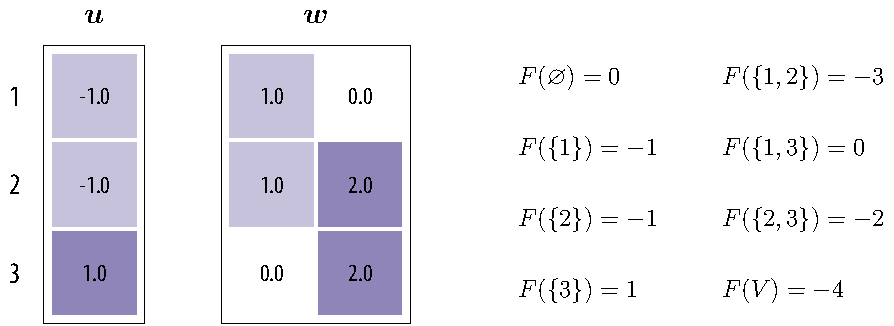
\includegraphics[width=0.9\textwidth]{figures/background/flid.pdf}
  \end{subfigure}\\[1.5em]
  \begin{subfigure}[b]{\subflen}
    \centering
    \hspace{-2.65em}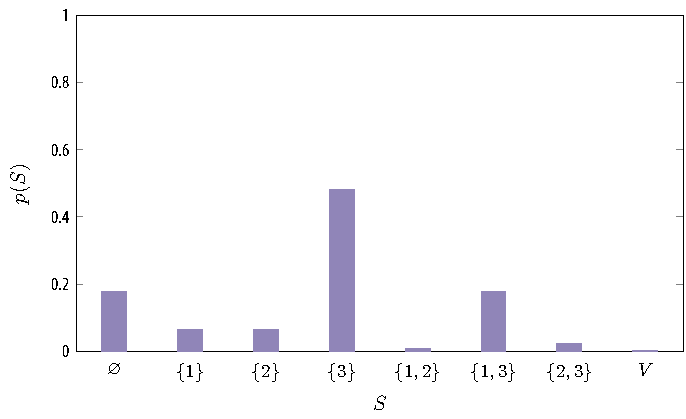
\includegraphics[width=1.07\textwidth]{figures/background/flid_dist.pdf}
  \end{subfigure}\\[1em]
  \caption{An example \flid{} model with $L = 2$ dimensions on ground set $V = \{1, 2, 3\}$, the corresponding values of the facility location function $F(S)$, for all $S \subseteq V$, and the resulting distribution $p(S) \propto \exp(F(S))$.}
  \label{fig:flid}
\end{figure}
\end{example}

\begin{example}[\fldc{}] \label{ex:fldc}
\cite{djolonga16mixed} extended the \flid{} model described above to include an additional matrix $\bv$ that encodes ``attraction'' between groups of elements.
The additional term is analogous to the original facility location function, except that its sign is reversed.
The corresponding function of the resulting facility location diversity and complements (\fldc{}) model is of the following form,
\begin{align*}
F(S) = \sum_{i \in S} u_i + \sum_{j=1}^{L} \left(\max_{i \in S} w_{ij} - \sum_{i \in S} w_{ij}\right) - \sum_{j=1}^{K} \left(\max_{i \in S} v_{ij} - \sum_{i \in S} v_{ij}\right).
\end{align*}
We have now $L$ latent dimensions encoding diversity or mutual exclusivity, and $K$ latent dimensions encoding complementarity or co-occurrence.
Note that the added term is a supermodular function, therefore $F(S)$ is neither submodular nor supermodular anymore.
It follows that the distribution $F(S) \propto \exp(F(S))$ is not a probabilistic submodular model.

In \figref{fig:fldc}, we show an example \fldc{} model, which has the same $\bu$ and $\bw$ as our previous \flid{} example, but additionally contains an attractive matrix $\bv$ of dimension $K = 1$.
The single latent dimension encodes co-occurrence between elements $1$ and $3$.
While the only function values that change from before are $F(\{1, 3\})$ and $F(V)$, note that all probabilities $p(S)$ are different than those of \figref{fig:flid}, because of the new partition function $Z$.

\renewcommand{\subflen}{\textwidth}
\begin{figure}[htbp]
  \centering
  \begin{subfigure}[b]{\subflen}
    \centering
    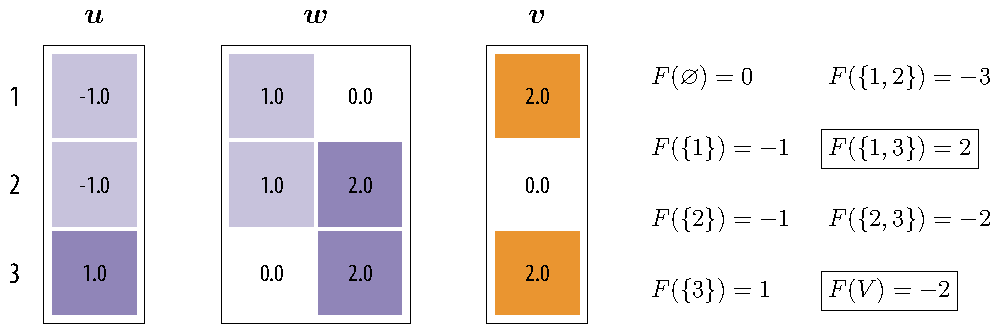
\includegraphics[width=\textwidth]{figures/background/fldc.pdf}
  \end{subfigure}\\[1.5em]
  \begin{subfigure}[b]{\subflen}
    \centering
    \hspace{-2.65em}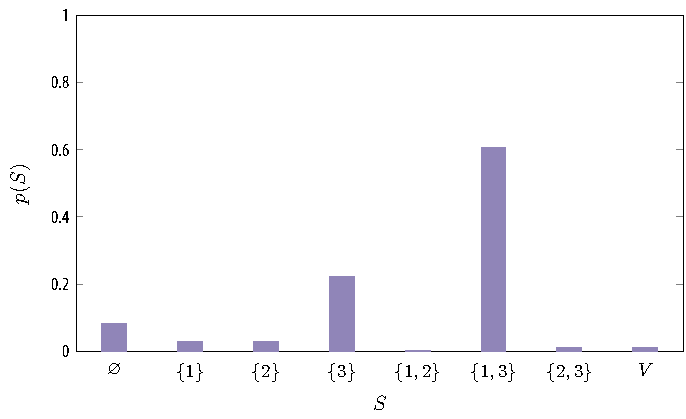
\includegraphics[width=1.07\textwidth]{figures/background/fldc_dist.pdf}
  \end{subfigure}\\[1em]
  \caption{An example \fldc{} model with $L = 2$ and $K = 1$ dimensions on ground set $V = \{1, 2, 3\}$, the corresponding values of $F(S)$, for all $S \subseteq V$, and the resulting distribution $p(S) \propto \exp(F(S))$.
  The two function values $F(\{1, 3\})$ and $F(V)$ are the only ones that change compared to the previous \flid{} example.
  }
  \label{fig:fldc}
\end{figure}
\end{example}


\subsection{Inference}
The basic tasks we would like to perform in a given discrete probabilistic model are computing various marginal probabilities of interest, and computing the partition function $Z$.
These two tasks are more often that not tightly related to each other, and many algorithms that accomplish one of them can also accomplish the other with minor modifications.
We therefore refer to them jointly as \emph{probabilistic inference}.
There are very few classes of discrete probabilistic models that are known to be amenable to tractable exact inference.
The most prominent such class are determinantal point processes that we described above.

On the other hand, is well known that performing exact inference in general probabilistic submodular models is a computationally intractable problem.
In fact, even for Ising models, \cite{jerrum93} showed that exactly computing the partition function is a \#P-hard problem.
Worse than that, they showed that there can be no FPRAS for these models unless RP = NP.
However, they also proposed a sampling-based procedure for performing approximate inference in ferromagnetic Ising models under some conditions.
Several other conditional results for approximate sampling-based inference are known for Ising models (Ch. 15, \citealp{levin08book}).
A generalization of determinantal point processes, called strongly Rayleigh distributions \citep{borcea08}, are the result of a long line of research into the notion of negative dependence between random variables \citep{pemantle00,liggett02,wagner08}.
It has been shown that one can efficiently sample from strongly Rayleigh distributions using a simple Metropolis sampler \citep{anari16,li16}.

\cite{iyer15} have considered a different class of probabilistic models, called submodular point processes, which are also defined via submodular functions, and are of the form $p(S) \propto F(S)$.
They showed that inference in SPPs is, in general, also a hard problem, and provided approximations and closed-form solutions for some subclasses.

Besides sampling, the primary alternative for performing approximate inference in discrete models have been variational methods.
The fundamental idea of these methods is to choose a distribution among a tractable class to approximate the true distribution at hand.
There has been extensive research on variational methods for low-order models, particularly for exponential families, and many well-known algorithms, such as belief propagation, or mean-field methods, fall under this category. (For an introductory treatment we refer to the monograph by \cite{wainwright08}.)
More recently, \citet{djolonga14} have proposed a variational approach for performing approximate probabilistic inference in probabilistic submodular models, based on log-modular approximations of the distribution.


\section{Sampling} \label{sect:sampling}
In this thesis, we focus on Markov chain Monte Carlo sampling algorithms, which are based on performing randomly selected moves in a state space $\ss$ to approximate probabilistic quantities of interest.
The visited states $(X_0, X_1,\ldots)$ form a Markov chain, which under mild conditions converges to a stationary distribution $p$ (see Theorem 4.9, \citealp{levin08book}).
Crucially, the probabilities of transitioning from one state to another are carefully chosen to ensure that the stationary distribution is identical to the distribution of interest.
In our case, the state space is the powerset of our ground set, that is, $\ss \defeq 2^V$, and we want to construct a chain over subsets of $V$ that has stationary distribution $p$.
We denote by $P : \Omega \times \Omega \to \mathbb{R}$ the transition matrix of a Markov chain, i.e., for all $S, R \in \Omega$, $P(S, R) \defeq \P\left[ X_{t+1} = R \,|\, X_t = S \right]$.

We next present two well-known chains that we will use throughout this thesis.
Both of them are by construction reversible with respect to $p(\cdot) \propto \exp(F(\cdot))$, that is, they satisfy the detailed balance conditions
\begin{align*}
p(S) P(S, R) = p(R) P(R, S),
\end{align*}
for all $S, R \in \ss$.
It follows that they asymptotically converge to the unique stationary distribution $p$.

\paragraph{Gibbs sampler.}
One of the most commonly used chains is the (single-site) Gibbs sampler, also known as the Glauber dynamics, which adds or removes a single element at a time.
It first selects uniformly at random an element $i \in V$; subsequently, it adds or removes $i$ to the current state $X_t$ according to the probability of the resulting state, as shown in \algoref{alg:gibbs}.
More concretely, we define an adjacency relation $S \sim R$ on the elements of the state space, which denotes that $S$ and $R$ differ by exactly one element, i.e., $\big||R| - |S|\big| = 1$.
It follows that each $S \in \ss$ has exactly $n$ neighbors.
We also define
\begin{align*}
p_{S \rightarrow R} = \displaystyle\frac{\exp(F(R))}{\exp(F(R)) + \exp(F(S))}.
\end{align*}
Then, the transition matrix $\Pg$ of the Gibbs sampler is
\begin{align*}
  \Pg(S, R) = 
  \threepartdefo{\displaystyle\frac{1}{n}p_{S \rightarrow R}}{R \sim S}{1 - \displaystyle\sum_{T \sim S} \displaystyle\frac{1}{n}p_{S \rightarrow T}}{R = S}{0}.
\end{align*}

In \figref{fig:gibbs} we illustrate one step of the Gibbs sampler on a small ground set $V = \{1, 2, 3\}$.
Assuming that the current state is $X_t = \{2\}$, there are three potential new next states, namely $\varnothing$, $\{1, 2\}$, or $\{2, 3\}$, which are the three neighbors of $X_t$ in the state space.
The Gibbs sampler first selects one of the neighbors uniformly at random, and then either stays at $X_t$ or moves to that neighbor according to the corresponding conditional probability.

\begin{algorithm}[p]
    \setstretch{1.3}
    \DontPrintSemicolon
	\caption{\strut The Gibbs sampler for probabilistic submodular models.}
	\label{alg:gibbs}
    \vspace{0.5em}
    \SetKwInOut{Input}{Input}
    \Input{Ground set $V$, distribution $p(\cdot) \propto \exp(F(\cdot))$}
	$X_0$ $\gets$ random subset of $V$\\
	\For{$t = 0$ \KwTo $M$}{
	  Draw $i \sim \mathrm{Unif}(V)$\;
	  $p_{\mathrm{add}}$ $\gets$ $\exp(\Delta_F(i \,|\, X_t))/(1 + \exp(\Delta_F(i \,|\, X_t)))$\;
	  Draw $z \sim \mathrm{Unif}([0,1])$\;
	  \uIf{$z \leq p_{\mathrm{add}}$}{
        $X_{t+1}$ $\gets$ $X_t \cup \{i\}$\;
      } \Else{
        $X_{t+1} \gets X_t \setminus \{i\}$\;
      }}
\end{algorithm}

\vspace{1em}
\begin{figure}[p]
\centering
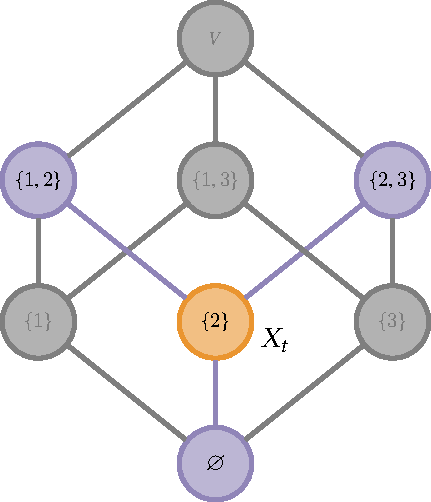
\includegraphics[width=0.5\textwidth]{figures/gibbs/lattice_gibbs_2.pdf}\\[1em]
\caption{An illustration of a single Gibbs step on ground set $V = \{1, 2, 3\}$, and current state $X_t = \{2\}$.
We first choose one of the neighbors of $X_t$ uniformly at random, and then either stay at $X_t$ or move to that neighbor according to the corresponding conditional probability.}
\label{fig:gibbs}
\end{figure}

It is important to note here that the computed conditional probabilities do not depend on the partition function $Z$, thus the chain can be simulated efficiently, even though $Z$ is unknown and hard to compute.
Moreover, it is easy to see that
\begin{align*}
\Delta_F(i \,|\, X_t) = \llbracket i\not\in X_t\rrbracket F(i \,|\, X_t) + \llbracket i\in X_t\rrbracket F(i \,|\, X_t\setminus\{i\}).
\end{align*}
Therefore, the Gibbs sampler only requires a black box for the marginal gains of $F$, which are often faster to compute in practice than the values of $F$ itself.
Finally, it is easy to show that the stationary distribution of the chain constructed this way is $p$.

\paragraph{Metropolis sampler.}
Another well-studied chain is the Metropolis chain \citep{metropolis,hastings}, which, like the Gibbs sampler, also performs local moves between neighboring states, but does so following a somewhat different procedure.
The Metropolis chain first draws a candidate next state according to a proposal distribution $q(\cdot\,|\,X_t)$; then, it either accepts the proposed state or not according to the probability ratio of the two states corrected by the proposal ratio, as shown in \algoref{alg:metropolis}.

\begin{algorithm}[tbp]
    \setstretch{1.3}
    \DontPrintSemicolon
	\caption{\strut The Metropolis sampler for prob. sub. models.}
	\label{alg:metropolis}
    \vspace{0.5em}
    \SetKwInOut{Input}{Input}
    \Input{Ground set $V$, distribution $p(\cdot) \propto \exp(F(\cdot))$, proposal $q$}
	$X_0$ $\gets$ random subset of $V$\\
	\For{$t = 0$ \KwTo $M$}{
	  Draw $S \sim q(\cdot \,|\, X_t)$\;
	  $p_{\textrm{acc}} \gets \min\left\{1, \frac{q(S \,|\, R)\,\exp(F(R))}{q(R \,|\, S)\,\exp(F(S))}\right\}$\;
	  Draw $z \sim \mathrm{Unif}([0,1])$\;
	  \uIf{$z \leq p_{\textrm{acc}}$}{
        $X_{t+1}$ $\gets$ $S$\;
      } \Else{
        $X_{t+1} \gets X_t$\;
      }}
\end{algorithm}

More concretely, if we define the acceptance probability
\begin{align*}
  p_{\textrm{acc}}(S, R) \defeq \min\left\{1, \displaystyle\frac{q(S \,|\, R)\,p(R)}{q(R \,|\, s)\,p(S)}\right\} = \min\left\{1, \displaystyle\frac{q(S \,|\, R)\,\exp(F(R))}{q(R \,|\, s)\,\exp(F(S))}\right\},
\end{align*}
then the transition matrix of the Metropolis chain can be defined as follows,
\begin{align*}
  \Pm(S, R) = \twopartdefo{q(R \,|\, S)\,p_{\textrm{acc}}(S, R)}{R \neq S\vspace{1em}}{1 - \displaystyle\sum_{T \neq S} q(T \,|\, S)\,p_{\textrm{acc}}(S, T)}.
\end{align*}
As with the Gibbs sampler, the computed acceptance probabilities do not depend on the partition function $Z$, therefore the chain can be simulated efficiently.

\paragraph{Approximating expectations.}
Approximating quantities of interest using MCMC methods is largely based on using time averages to estimate expectations over the desired distribution.
In particular, we estimate the expected value of function $g : \ss \to \mathbb{R}$ by
\begin{align} \label{eq:exp_approx}
\E_p[g(X)] \approx \frac{1}{M}\sum_{r=1}^{M} g(X_{s + r}).
\end{align}
The point in time $s \in \mathbb{N}$, after which we start taking samples into account, is often referred to as the burn-in time of the chain.
For example, to estimate the marginal probability $\P(i \in S)$, for some $i \in V$, we would define $g(S) = \llbracket i \in S \rrbracket$, for all $S \in \ss$.

\paragraph{Approximating the partition function.}
There are two straightforward methods for estimating the partition function $Z$ using sampling.
The first, importance sampling (IS) \citep{ais}, assumes that we have a tractable distribution $\pi : 2^V \to \mathbb{R}$, from which we draw $M$ samples $\{x_{s+1}, \ldots, x_{s+M}\}$.
Then, we can estimate the partition function of $p(\cdot) \propto \exp(F(\cdot))$ by
\begin{align} \label{eq:is}
Z_{\textrm{IS}} \defeq \frac{1}{M} \sum_{r = 1}^{M} \frac{\exp(F(x_{s+r}))}{\pi(x_{s+r})}.
\end{align}
Although this is known to be an unbiased estimator of $Z$, it often has high variance, and tends to underestimate the true value of the partition function.

The second method, reverse important sampling (RIS) \citep{ris}, works in the opposite direction, by first sampling $M$ samples $\{x_{s+1}, \ldots, x_{s+M}\}$ from the target distribution $p$, and then estimating the partition function by
\begin{align} \label{eq:ris}
Z_{\textrm{RIS}} \defeq \left(\frac{1}{M} \sum_{r = 1}^{M} \frac{\pi(x_{s+r})}{\exp(F(x_{s+r}))}\right)^{-1}.
\end{align}
Similarly to the IS estimator, the RIS estimator also often has high variance, but it tends to overestimate the true value of the partition function.
Taking the average $0.5 Z_{\textrm{IS}} + 0.5 Z_{\textrm{RIS}}$ is then a natural way to obtain an estimate, while other more involved related methods have also been proposed \citep{burda15,liu15}.

\paragraph{Mixing time.}
The choice of burn-in time $s$ and number of samples $M$ in \eqref{eq:exp_approx}--\eqref{eq:ris} presents a tradeoff between computational efficiency and approximation accuracy.
It turns out that the effect of both $s$ and $M$ is largely dependent on a fundamental quantity of the chain called \emph{mixing time} \citep{levin08book}.

The mixing time of a chain quantifies the number of iterations $t$ required for the distribution of $X_t$ to get close to the stationary distribution $p$.
More formally, it is defined as
\begin{align*}
\tme \defeq \min \sdef{t}{d(t) \leq \epsilon},
\end{align*}
where $d(t)$ denotes the worst-case (over the starting state $X_0$ of the chain) total variation distance between the distribution of $X_t$ and $\pi$, that is,
\begin{align*}
d(t) \defeq \max_{X_0 \in \ss} \| P^t(X_0, \cdot) - p \|_{\mathrm{TV}}.
\end{align*}
A generalization of Chebyshev's inequality to correlated Markov chain samples (see Theorem 12.19, \citealp{levin08book}) shows that upper bounding the mixing time is sufficient to guarantee efficient approximate sampling-based marginal inference.